\documentclass[12pt, a4paper]{article}

\usepackage{amsmath}
\usepackage[utf8]{inputenc}
\usepackage[spanish]{babel} %Paquete de idioma
\usepackage[hidelinks]{hyperref}
\usepackage{graphicx}
\usepackage{float}
\usepackage{eso-pic}
\usepackage{lipsum}
\usepackage{transparent}
\usepackage{parskip}
%\usepackage[backend=biber, style=apa]{biblatex}

\graphicspath{{imagenes/}}

%%%%%%%%% ESTO PARA LA MARCA DE AGUA %%%%%%%%%%%%%%%%%%%%%%%%%%%%%%%


\AddToShipoutPicture{ 
    \put(410,380){
        \parbox[b][\paperheight]{\paperwidth}{%
            \vfill
            \
            {
            \transparent{1}
            
\includegraphics[scale=0.5]{logo-ua.png}
            \vfill
            }
        }
    }
}
%%%%%%%%%%%%%%%%%%%%%%%%%%%%%%%%%%%%%%%%%%%%%%%%%%%%%%%%%%

\title{Memoria Práctica 2 \\


\large Comunicaciones
}
\author{
Leopoldo Cadavid Piñero
}
\date{Febrero 2022}







\begin{document}

\maketitle
\newpage
\tableofcontents
\newpage
\section{Introducción}
      
En la siguiente práctica continuaremos con el aprendizaje distintos tipos de plataformas que nos permitan realizar aplicaciones del 
tipo IOT, así como el reforzamiento con herramientas como Nodered o la introducción a nuevos tipos de protocolos de comunicaciones 
como lo puede ser el MQTT. 

\section{Sesión 1: Ubidots}
El objetivo en esta sesión es instalar y familiarizarse con la plataforma Ubidots. Ubidots es una plataforma de gestión de módulos enfocada para 
trabajar el campo de \textit{Internet of Things}. En la práctica lo que haremos será loguear en la página y utilizar la API para trabajar desde Nodered.

Lo primero será registrarse en la página y crear lo que se llama en la plataforma \textit{"Devices"}. Obtenemos un token para comunicarnos con Nodered, y 
nos vamos a crear el siguiente Nodo:

\begin{figure}[H]
    \centering
    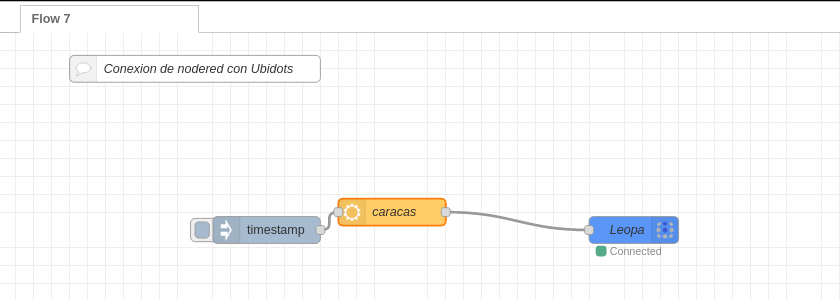
\includegraphics[scale=0.4]{nodered_ubidots.png}
    \caption{Nodo básico de Conexión entre Ubidots, Nodered y OpenWeather}
\end{figure}

Si vamos a Ubidots, veremos lo siguiente: 

\begin{figure}[H]
    \centering
    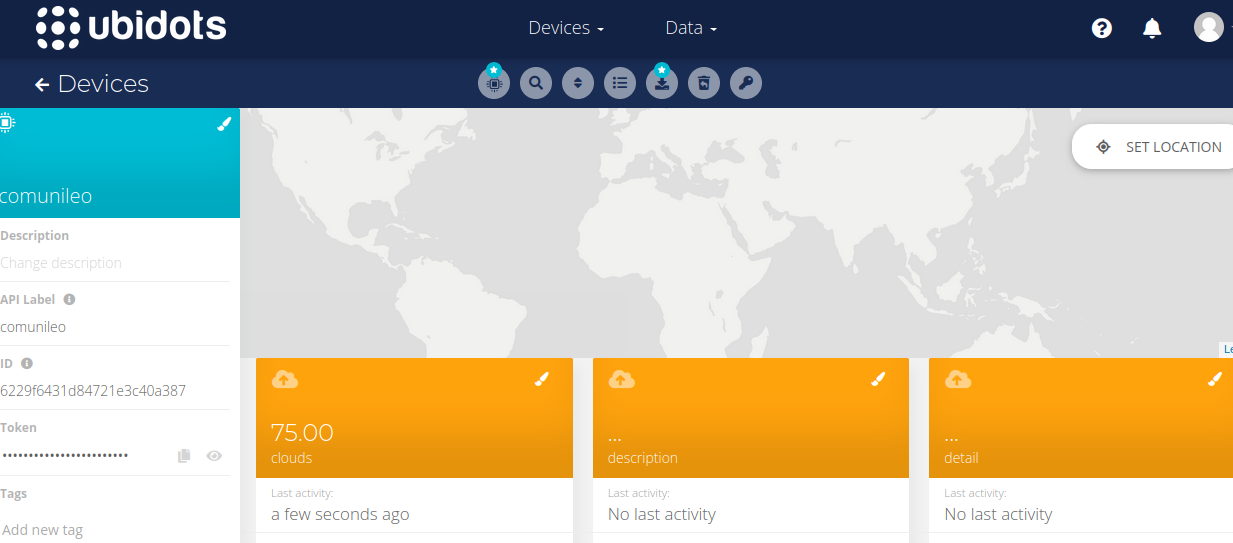
\includegraphics[scale=0.3]{deviceprimero.png}
    \caption{Resultado de la variable de Ubidots}
\end{figure}

En la anterior imagen vemos cómo en ubidots hemos recibido varias de las variables que nos proporciona el nodo de OpenWeather. 

Ahora, a modo de ampliación, lo que haremos es filtrar la información que enviamos desde Nodered, para que sólo reciba la variable temperatura, y además para que 
esta se encuentre en centígrados. Para ello debemos escribir una función que recoja y envíe específicamente ese parámetro en el formato necesario para que lo lea 
la API de Ubidots. El nodo sería el siguiente:

\begin{figure}[H]
    \centering
    \includegraphics[scale=0.5]{ampliacion_añadir_parametroenjson.png}
    \caption{Nodo de ampliacion de Ubidots}
\end{figure}

Finalmente, con el valor de la temperatura que recogemos en Ubidots, creamos un dashboard para ejemplificar el potencial de la plataforma
en cuanto a gestión de información y automatización. El resultado sería el siguiente:

\begin{figure}[H]
    \centering
    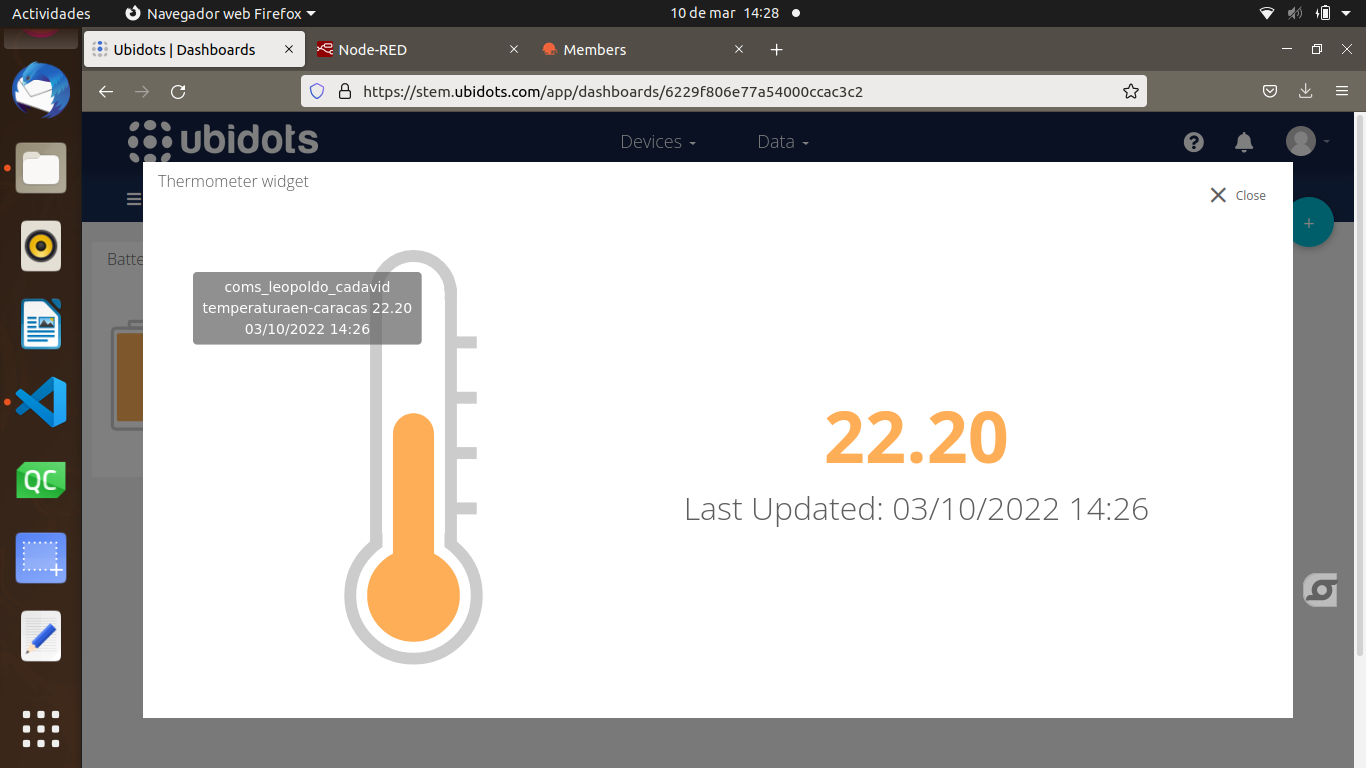
\includegraphics[scale=0.29]{Captura de pantalla de 2022-03-10 14-28-16.png}
    \caption{Nodo de ampliacion de Ubidots}
\end{figure}

\section{Sesión 2: Introducción al entorno de Shelly}

En esta sesión lo que haremos será iniciar el proceso de automatización de una sencilla instalación, usando protocolos de comunicación vistos en la teoría.
    
Lo que haremos en esta primera sesión será principalmente seguir los pasos que realiza el compañero para conectarse a la instalación.    

Los pasos seguidos en clase han sido:
\begin{itemize}
    \item Conectarse a la red del router de la instalación que es la subred de control
    \item Meterse en la  interfaz de shelly
    \item Desde aquí podremos conectarnos a los dispositivos del sistema y probar como podemos dar instrucciones y recibir info
    \item \textbf{Aconsejable:} decirle al shelly a que red se tiene que conectar. Decimos a shelly que se conecte a la red que nosotros queremos
    (esto se graba en su memoria).
    \item Para nuestro caso: \textbf{Nombre de la red:} Cudy-081c, \textbf{IP:} 192.168.10.100 (rango x.x.10.(0/255)), 
    \textbf{Gateway (opcional):}. 
    \item Si hemos introducido todo bien, nuestro shell estará conectado en la red del router.
    \item Necesitamos saber las peticiones get para acceder a los componentes.
    \item En clase el compañero se ha conectado a la ip comentada y ha encendido y apagado el relé de la instalación.
    

\end{itemize}

No se llegaron a especificar más objetivos para esta sesión.

\section{Sesión 3: Uso del protocolo HTTP Request}

En esta sesión proseguiremos con el aprendizaje de protocolos sobre la instalacióny para ello haremos uso de las peticiones
por http, los bloques \textit{HTTP Request} del Nodered.

El profesor nos da especificaciones y seguimos los siguientes pasos: 
\begin{itemize}
    \item \textbf{Red:} Cudy-081c ,  \textbf{Clave:} Comunica2022
    \item Nos conectamos a la IP: 192.168.10.100
    \item \textbf{Peticiones:} nos metemos en Nodered y con el 
    nodo \textit{http request} con el método \textbf{get y url 192.168.10.110/relay/0?turn=off}. Con esto, nos conectaremos al relé de 
    la estación de clase y podemos encender o apagar el relé según consideremos. 
 
\end{itemize}

Primero, veamos el entorno de shelly al estar conectados a la red de Cudy:

\begin{figure}[H]
    \centering
    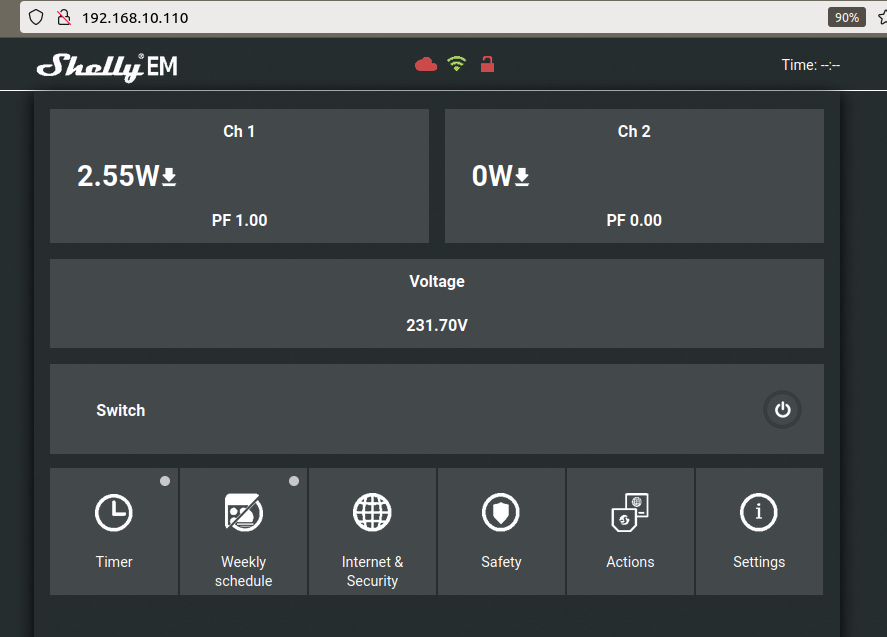
\includegraphics[scale=0.4]{conexionaashely.png}
    \caption{Vista de la interfaz Shelly}
\end{figure}

Ahora veamos los nodos implementados en Nodered para realizar la conexión de este con el Shelly.

\begin{figure}[H]
    \centering
    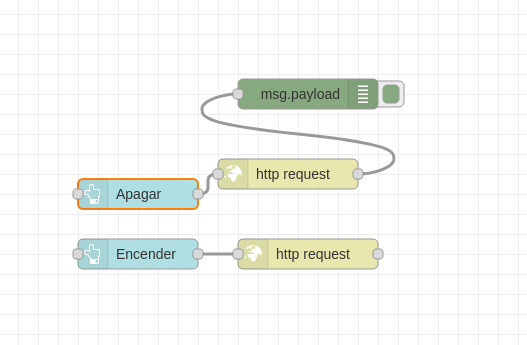
\includegraphics[scale=0.5]{Botones_con_flow.png}
    \caption{Nodos con protocolo HTTP request}
\end{figure}

Y el resultado en la UI  de Nodered:

\begin{figure}[H]
    \centering
    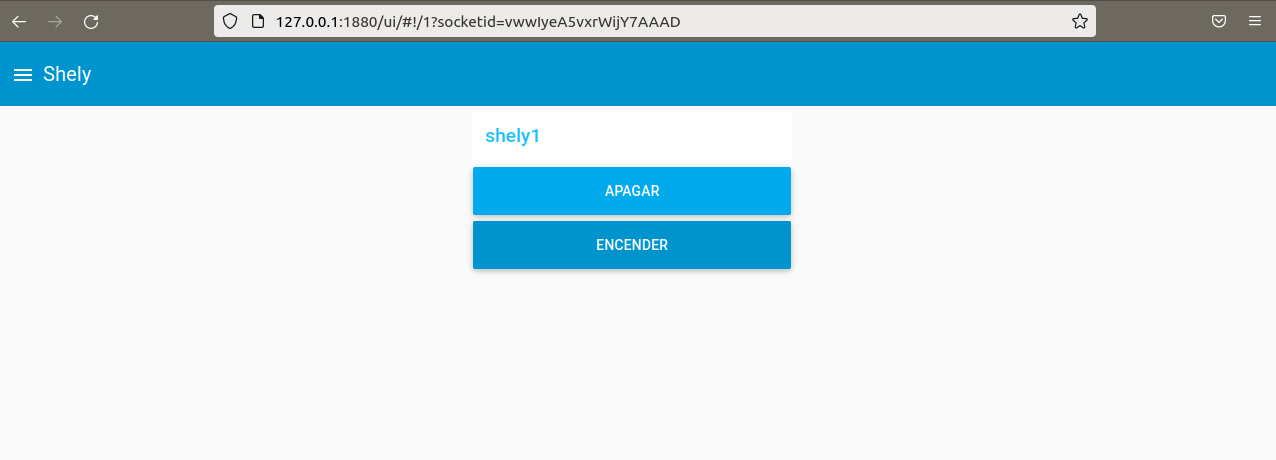
\includegraphics[scale=0.3]{botones_ui_nodered.png}
    \caption{Interfaz de los botones}
\end{figure}

Adicionalmente lo que se ha hecho es introducir una interfaz para visualizar el estado de nuestro relé en tiempo real. Esto lo 
hacemos con un código que trate el mensaje que recibimos del estado del relé, que puede ser \verb|"On"| u \verb|"Off"|. 
El nodo y los resultados son los siguientes:

\begin{figure}[H]
    \centering
    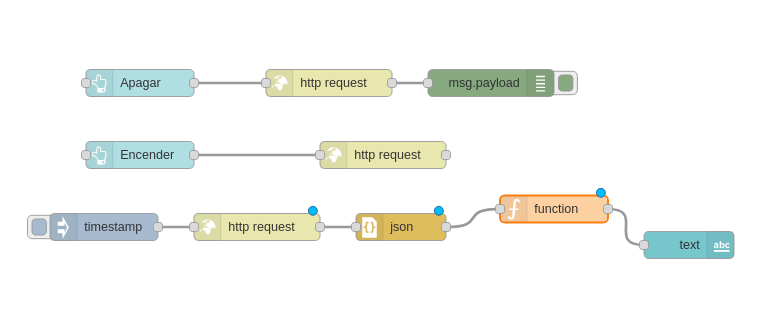
\includegraphics[scale=0.5]{botones_y_lectura.png}
    \caption{Botones y lectura del relé}
\end{figure}

\begin{figure}[H]
    \centering
    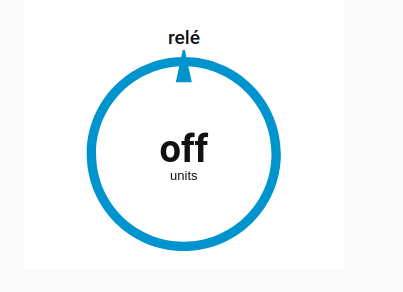
\includegraphics[scale=0.5]{dashboarestadorele.png}
    \caption{Visualización del estado del relé, en tiempo real}
\end{figure}

\section{Sesión 4: Uso del MQTT}

La idea de esta sesión es cambiar el uso de http requests, por 
el uso de nodos mqtt, para que la carga de las conexiones recaiga sobre
el broker, en este caso la raspberry, en vez de en el shelly. Este protocolo resulta interesante porque permite un
mayor tráfico de información sobre la instalación, dejando que un sistema más potente se encarge de publicar la información a 
otros suscriptores que la necesiten, pero sin que la propia Shelly deba saturarse por la carga de trabajo.


Algunos pasos seguidos en la sesión:

\begin{itemize}
    \item creamos nodo mqtt
    \item Debemos configurar info del broker: Clave: comunicacionespass;
    IP: 192.16810.144
    \item configuramos el topic según los intereses 
\end{itemize}

El siguiente paso de la sesión será ver como podemos ver el topic del
shelly donde se estan publicando los datos que nos interesen. Veamos el flow de Nodered implementado 
para tal proposito:

\begin{figure}[H]
    \centering
    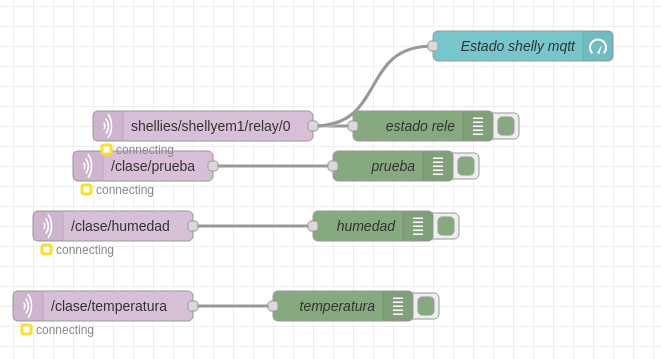
\includegraphics[scale=0.5]{mqttconvisualiz.png}
    \caption{Shelly con protocolo MQTT}
\end{figure}

Vemos en la anterior imagen cómo estamos accediendo a los datos de: humedad, temperatura, o estado del relé de nuestra instalación,
todo suscribiendonos a los topics correspondientes. Algunas lecturas vistas desde el debugger:

\begin{figure}[H]
    \centering
    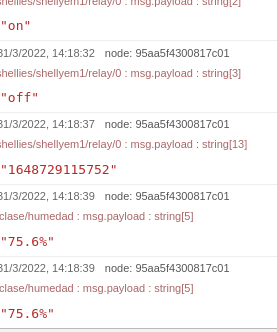
\includegraphics[scale=0.7]{Captura de pantalla de 2022-03-31 14-18-35.png}
    \caption{Resultados de la lectura de los topics}
\end{figure}

\begin{figure}[H]
    \centering
    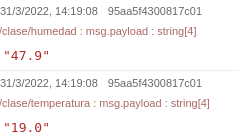
\includegraphics[scale=0.8]{Captura de pantalla de 2022-03-31 14-19-14.png}
    \caption{Resultados de la lectura de los topics}
\end{figure}

A modo de añadido, se ha introducido la interfaz de encendido y apagado de botones que se utilizó en el apartado anterior, pero adaptado 
al protocolo MQTT.

\begin{figure}[H]
    \centering
    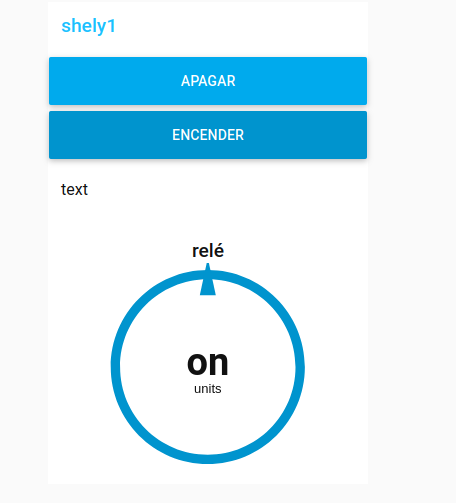
\includegraphics[scale=0.8]{estadoreleybotones.png}
    \caption{UI conectada a los topics MQTT}
\end{figure}



\section{Ampliaciones finales}

Finalmente, a modo de ampliación final, siguiendo con lo visto en la anterior práctica, se ha desarrollado un flow de 
Nodered, que se conecte a la Api de telegram para que podamos encender y apagar el relé desde la aplicación, además, podremos consultar la temperatura
de la estación desde el móvil. 

El flow desarrollado ha sido el siguiente:

\begin{figure}[H]
    \centering
    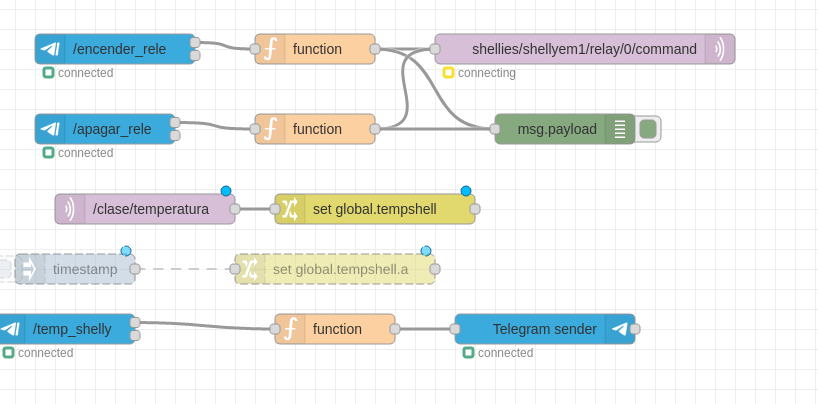
\includegraphics[scale=0.5]{ampliaciontelegram.png}
    \caption{Ampliación usando API de Telegram en Nodered}
\end{figure}

Los comandos creados han sido \textbf{/encender\_rele}, \textbf{/apagar\_rele}
 y \textbf{/temp\_shelly}. Para encender y apagar el relé, simplemente esperamos a recibir el comando, en cuyo caso,
vamos al topic \textbf{"shellies/shellyem1/relay/0/command"} y publicamos el estado que corresponda usando 
\verb|"On"| u \verb|"Off"|.

Para la lectura de la temperetura, la estrategia es conectarse al topic de shelly que corresponde y recibir constantemente 
la información, la cual guardamos en una variable global a la que accederemos desde otro nodo, cuando se  requiera publicar esta información.
Así evitaremos estar publicando constantemente el valor de la temperatura en Telegram, pero nos aseguraremos de tener el valor más actual posible 
una vez haya sido pedido este.

Es importante mencionar que, aunque se ha implementado el nodo y realizado algunas pruebas, resulta físicamente imposible realizar una prueba con 
la instalación de la cual disponemos en el laboratorio, esto se debe a que, para poder ver lo que publica Shelly, debemos estar conectados al router del laboratorio,
lo cual nos imposibilita estar conectados al wifi y poder realizar la conexión con Telegram. Para poder realizar algo parecido,deberiamos conseguir conectar el Shelly a internet, como indicaba
el profesor en la sesión 2. Para ello, habría que incicar a Shelly una red para conectarse y esta quedará grabada en su memoria.

Ahora bien, realizando algunas emulaciones podemos ver si al menos la lógica por la cuá se ha implementado el flow esta bien encaminada. Por ejemplo, si escribimos
los comandos para encender y apagar el relé en Telegram, y posteriormente visualizamos mediante el debugger lo que se publicaría al topic vemos lo 
siguiente:

\begin{figure}[H]
    \centering
    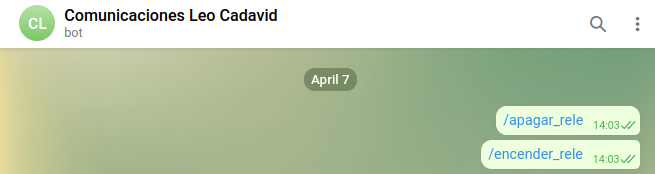
\includegraphics[scale=0.5]{telegram_encender_apagar.png}
    \caption{Comandos dados al bot en Telegram}
\end{figure}

\begin{figure}[H]
    \centering
    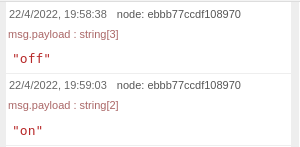
\includegraphics[scale=0.5]{resultadoencenderapagar.png}
    \caption{información que se publica al topic que enciende y apaga el relé}
\end{figure}

Como observamos, en caso de encontrarse conectado a la vez a Shelly y a Telegram, los mensajes correctos se estarían publicando al topic,
permitiéndonos encender y apagar el relé desde la aplicación.

En el caso de revisar la temperatura, podemos sustituir el mensaje a recibir del topic, por un timestamp con un número prefijado a modo de 
simulación de la temperatura. Si hacemos esto, y ejecutamos el comando en Telegram podemos ver lo siguiente:

\begin{figure}[H]
    \centering
    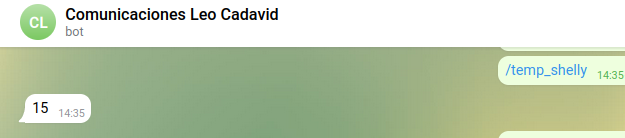
\includegraphics[scale=0.5]{tempshelly.png}
    \caption{Temperatura simulada de la instalación}
\end{figure}

Vemos que si llegamos a recibir la información, y en caso de estar conectados a Shelly, solo haría falta cambiar el timestamp
por un nodo \textit{mqtt in}.

\end{document}

